% *********************************************************************
% © 2026 Jeremy Sylvestre
%
% Permission is granted to copy, distribute and/or modify this document
% under the terms of the GNU Free Documentation License, Version 1.3 or
% any later version published by the Free Software Foundation; with no
% Invariant Sections, no Front-Cover Texts, and no Back-Cover Texts. A
% copy of the license is included in the appendix entitled “GNU Free
% Documentation License” that appears in the output document of this
% PreTeXt source code. All trademarks™ are the registered® marks of
% their respective owners.
%
% *********************************************************************
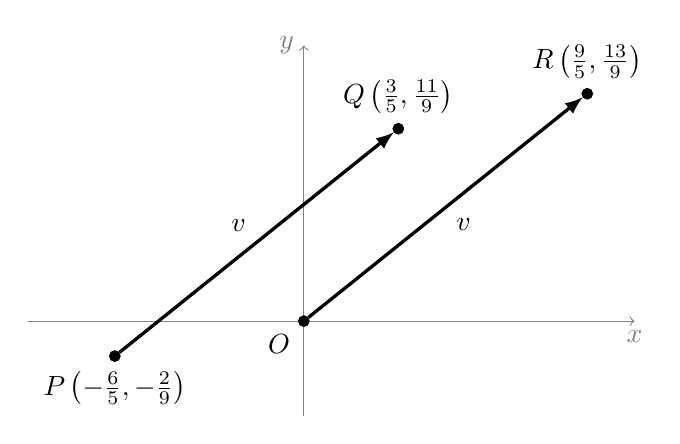
\begin{tikzpicture}[
	point/.style={circle,draw,very thin,fill,inner sep=0pt,minimum size=4pt},
	vector/.style={-latex,very thick},
	scale=2
]
	\draw[gray,->] (-1.75,0) to (2.1,0) node[below] {$x$};
	\draw[gray,->] (0,-0.6) to (0,1.75) node[left] {$y$};

	\node[point] at (0,0) (o) [label=below left:$O$] {};
	\node[point] at (-1.2,-0.222) (p) [label=below:{$P\left(-\frac{6}{5},-\frac{2}{9}\right)$}] {};
	\node[point] at (0.6,1.222) (q) [label=above:{$Q\left(\frac{3}{5},\frac{11}{9}\right)$}] {};
	\draw[vector] (p) to node[above left] {$\uvec{v}$} (q);
	\node[point] at (1.8,1.444) (r) [label=above:{$R\left(\frac{9}{5},\frac{13}{9}\right)$}] {};
	\draw[vector] (o) to node[below right] {$\uvec{v}$} (r);

\end{tikzpicture}
